\documentclass[10pt,twocolumn]{IEEEtran}
% replace the keyword "twocolumn" by "onecolumn" if you want a single column document

% ------------------------------------------------------------------------------------
% If you are using *TeXnicCenter*, already configured with profiles as "LaTeX -> PDF",
% do the following to create a project and have the compile hotkey Ctrl+F5:
%     Project -> Create with active file as the main file
% Do not forget to select "Uses BibTeX"
% ------------------------------------------------------------------------------------

% some useful packages:
\usepackage{graphicx}
\graphicspath{{./}{./figs/}{../figs/}{../figs/w14/}} % share figs using ../figs/
\usepackage{url}
\usepackage{amsmath}

\begin{document}

\title{Report on proposed integration of FUSION and EKLT}
\author{Jose Pedro Gomes}

\maketitle

\begin{abstract}
    Documentation on the techniques suggested to combine the information between FUSION and EKLT, thus creating a closed loop.
\end{abstract}

\section{Introduction}

Tracking using events is not as robust as their full frame equivalents. There are no descriptors (as with SIFT/SURF) nor neighbouring information (as in Sum of Squared Errors) to help with tracking, and event feature tracking is mostly based on their high refresh rate, and subsequent small displacements. Nevertheless, features are eventually lost, and without new frames to extract new features (due to the hardware limitations of the DVS240 being used), no replacements are available. We try to help the feature tracking by keeping track the landmarks, even when their corresponding features have been lost, so that they can be later tracked, being placed in a temporary dormant state.

\section{FUSION}

FUSION is a UKF that relies on IMU and visual information to estimate the rotation, position, velocity, 3D landmark positions, and IMU sensor biases, according to the Lie group structure \eqref{eq:w14_state}, with the biases being appended to the state.

\begin{equation}
    \label{eq:w14_state}
    \chi = \begin{bmatrix}
        R & v & x & p_1 \cdots p_p \\ 
         &0_{2+p\times 3}   &&I_{p+2\times p+2}
        \end{bmatrix}
\end{equation}

In order to keep track of the state, FUSION uses IMU information (namely linear acceleration and angular velocity) as input to the motion model and the predict step, and combines this information with visual cues for the measurement model in the update step.

Combining these two types of information allows for a smoother and more robust state estimation (periods where visual information is scarce can be compensated by using the IMU information, for example).

\section{EKLT}

EKLT is a feature detector and tracker that combines frames and events. Frames share two purposes: detect features (using a Harris corner detector) and provide a template for feature location estimation. Events are used to track the features, by comparison of their region of interest to the template provided by the equivalent region in the frame (patch comparison).

The tracker relies on and provides information on the feature current estimated position, and its optical flow.

\section{Information sharing}

We propose an implementation where information is shared between FUSION and EKLT, leveraging the estimation being generated by each software, thus creating a sort of closed loop system where there is a synergy between the pose estimation and the feature tracking.

\subsection{EKLT $\rightarrow$ FUSION}

EKLT is influence on FUSION is obvious and crucial in the sense that the features being tracked by EKLT are used as the measurement update in the UKF. 

Better visual information should provide a better estimation of the state, and it is desirable to have many features being tracked (as too few can introduce noise).

\subsection{FUSION $\rightarrow$ EKLT}

FUSION can be used to help EKLT in the tracking of features. The estimated position and flow angle are estimated by visual information only. FUSION, on the other hand, has a state estimation \eqref{eq:w14_state} that includes the camera pose and the 3D position of the landmarks. This information can be fed into EKLT to improve its estimation. In particular, using a projection camera model we can provide the feature position in camera space (as estimated by EKTL), and using the motion field from ego-motion we can also obtain the flow angle (as estimated by EKTL as well).

Indeed, the feature position can be estimated by projecting its corresponding 3D landmark position according to \eqref{eq:w14_proj}.

\begin{equation}
    \label{eq:w14_proj}
    \lambda \begin{bmatrix}
        x_u^i\\ 
        y_u^i\\ 
        1
        \end{bmatrix}
        =
        \Pi \left[
        \mathbf{R}_C^T\left(\mathbf{R}^T\left(\mathbf{p}_i-x
         \right ) -x_c
         \right )
         \right ]
\end{equation}

Likewise, the optical flow can be approximated from the ego-motion, as shown in \eqref{eq:w14_flow}

\begin{equation}
    \label{eq:w14_flow}
    \begin{bmatrix}
        \dot{x}\\ 
        \dot{y}
        \end{bmatrix}
        =
        \frac{f}{Z}
        \begin{bmatrix}
            -T_x+\frac{x}{f}T_z\\ 
            -T_y+\frac{y}{f}T_z
            \end{bmatrix}
            +
            \begin{bmatrix}
                \omega_x \frac{xy}{f}-\omega_y\left( f + \frac{x^2}{f}\right) + \omega_z y\\ 
                \omega_x\left( f + \frac{y^2}{f}\right) - \omega_y \frac{xy}{f} + \omega_z x
            \end{bmatrix} 
\end{equation}

\begin{figure}[ht]
    \centering
    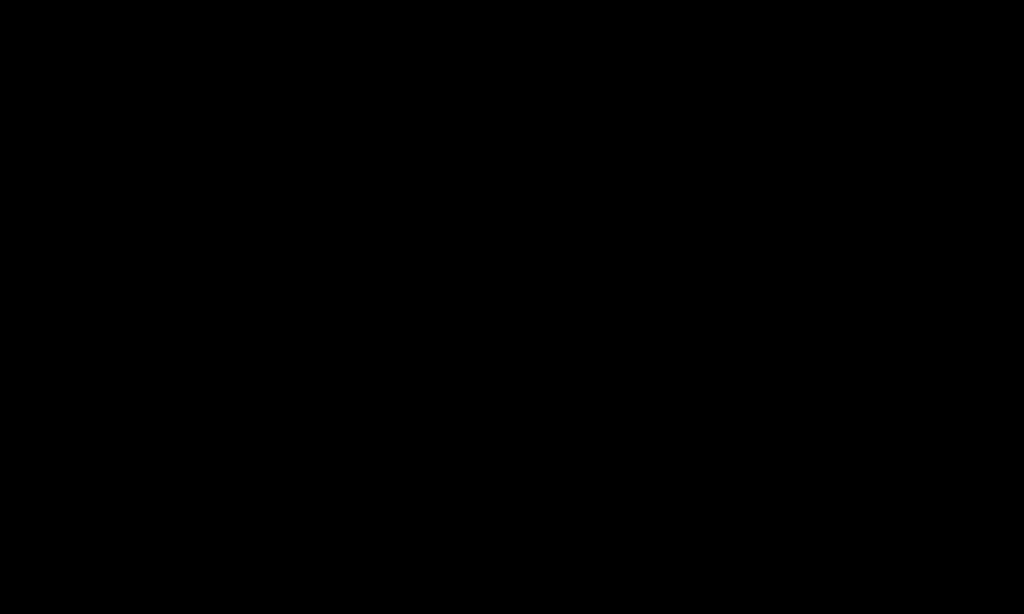
\includegraphics[width = 1\linewidth]{placeholder.png}
    \caption[]{placeholder}
    \label{placeholder}
\end{figure}




%\bibliographystyle{plain}
%\bibliography{../thesis/ref}
% replace "project" by "thesis" if you are doing the thesis

\end{document}
